%%==================================================
%% chapter03.tex for SJTU Bachelor Thesis
%% version: 0.5.2
%% Encoding: UTF-8
%%==================================================

% \bibliographystyle{sjtu2} %[此处用于每章都生产参考文献]

\chapter{避障算法的仿真}
\label{chap:simulation}
关于移动化机器人底盘系统的设计说明已经在前三章完成,在本章将对于算法的仿真做以详细的介绍。因为机器人的控制算法相对复杂,同时又涉及到在三维空间内的避障,所以一定要先进性动力学仿真,来验证算法的可行性。

\section{仿真软件环境介绍}
本设计将会使用GAZEBO动力学仿真环境来对在设计中出现的算法进行仿真。Gazebo是一个多机器人仿真环境,目前软件有能力在三维环境中仿真已有的多种机器人,传感器和其他物体。 在仿真环境里,可以模拟生成传感器返回量和根据物理引擎来模拟物体之间的相互作用,其尤为擅长对于刚体物理特性的仿真。GAZEBO具有一种分布式的结构,它的功能被封装在不同的库中,如物理仿真引擎,渲染,UI,通讯和传感器生成。在仿真中将涉及三个不同的部分:物理仿真,传感器生成,GUI界面,最后再加上一个全局坐标管理其。
\begin{figure}[!htp]
  \centering
  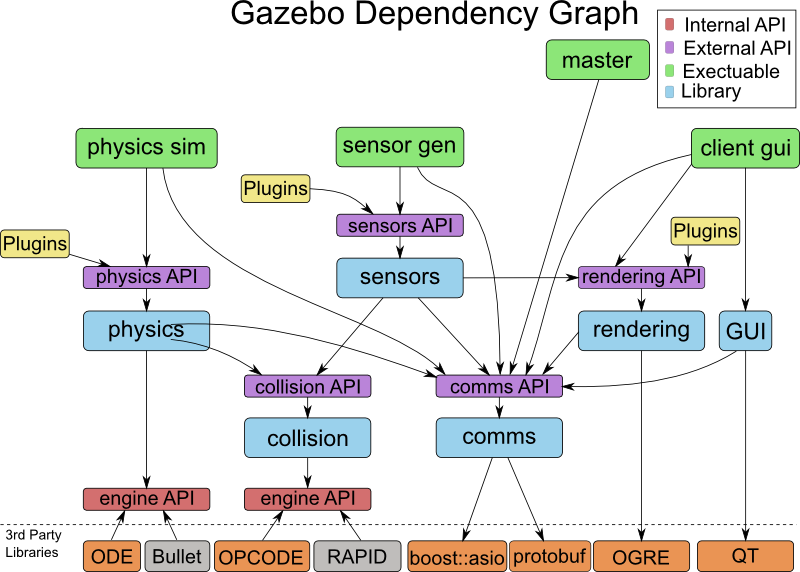
\includegraphics[width=0.8\textwidth]{chap5/Gazebo_design.PNG}
  \bicaption[fig.gazeboStructure]{GAZEBO系统结构图}{GAZEBO系统结构图}{Fig}{GAZEBO system diagram}
\end{figure}
\section{移动机器人模型的建立}
在GAZEBO中,所有机器人模型都是通过通用SDF文件来描述的,SDF文件是一个符合标准XML协议的文件。对于一个模型的描述包括四个个部分:Link,包含着一个物理模型的物理性质信息;collision,一个collision包含着一个需要检查碰撞的空间,同时其还有创建可视图形,定义惯性和粘连传感器;joint,定义了可以相对移动的不同部分的连接部分;组件,是一个公用库,定义了如何控制模型的方法。

对于本设计的机器人,因为要进行三维的碰撞检查,所以需要定义一个需要检查的空间;同时因为还有避障的需求,所以要在机器体上粘接12个超声波传感器;机器人是靠两个轮子进行驱动,因此还要加入两个驱动轮和一个万向轮。依据这些要求,说建立的机器人模型为 \\
\begin{lstlisting}[language={XML}, caption={机器人模型描述文件}]
<?xml version='1.0'?>
<sdf version='1.3'>
  <model name="my_robot">
    <link name='chassis'>
      <pose>0 0 .1 0 0 0</pose>
      <collision name='collision'>
        <geometry>
          <box>
            <size>.4 .2 .1</size>
          </box>
        </geometry>
      </collision>

      <visual name='visual'>
        <geometry>
          <box>
            <size>.4 .2 .1</size>
          </box>
        </geometry>
      </visual>

      <collision name='caster_collision'>
        <pose>-0.15 0 -0.05 0 0 0</pose>
        <geometry>
          <sphere>
          <radius>.05</radius>
        </sphere>
      </geometry>

      <surface>
        <friction>
          <ode>
            <mu>0</mu>
            <mu2>0</mu2>
            <slip1>1.0</slip1>
            <slip2>1.0</slip2>
          </ode>
        </friction>
      </surface>
    </collision>

    <visual name='caster_visual'>
      <pose>-0.15 0 -0.05 0 0 0</pose>
      <geometry>
        <sphere>
          <radius>.05</radius>
        </sphere>
      </geometry>
    </visual>
  </link>     
  <link name="left_wheel">
    <pose>0.1 0.13 0.1 0 1.5707 1.5707</pose>
    <collision name="collision">
      <geometry>
        <cylinder>
          <radius>.1</radius>
          <length>.05</length>
        </cylinder>
      </geometry>
    </collision>
    <visual name="visual">
      <geometry>
        <cylinder>
          <radius>.1</radius>
          <length>.05</length>
        </cylinder>
      </geometry>
    </visual>
  </link>

  <link name="right_wheel">
    <pose>0.1 -0.13 0.1 0 1.5707 1.5707</pose>
    <collision name="collision">
      <geometry>
        <cylinder>
          <radius>.1</radius>
          <length>.05</length>
        </cylinder>
      </geometry>
    </collision>
    <visual name="visual">
      <geometry>
        <cylinder>
          <radius>.1</radius>
          <length>.05</length>
        </cylinder>
      </geometry>
    </visual>
  </link>
  <joint type="revolute" name="left_wheel_hinge">
    <pose>0 0 -0.03 0 0 0</pose>
    <child>left_wheel</child>
    <parent>chassis</parent>
    <axis>
      <xyz>0 1 0</xyz>
    </axis>
  </joint>

  <joint type="revolute" name="right_wheel_hinge">
    <pose>0 0 0.03 0 0 0</pose>
    <child>right_wheel</child>
    <parent>chassis</parent>
    <axis>
      <xyz>0 1 0</xyz>
    </axis>
  </joint>
   </model>

  <include>
     <uri>model://ultrasonic</uri>
     <pose>0.2 0 0.2 0 0 0</pose>
  </include>
  <joint name="ultrasonic_joint" type="revolute">
    <child>hokuyo::link</child>
    <parent>chassis</parent>
    <axis>
      <xyz>0 0 1</xyz>
      <limit>
        <upper>0</upper>
        <lower>0</lower>
      </limit>
    </axis>
  </joint>  
</sdf>
\end{lstlisting}
配置文件为 \\
\begin{lstlisting}[language={XML}, caption={机器人模型配置文件}]
<?xml version="1.0"?>
<model>
  <name>My Robot</name>
  <version>1.0</version>
  <sdf version='1.3'>model.sdf</sdf>

  <author>
   <name>Cui Yunkai</name>
   <email>tccyk@sjtu.edu.cn</email>
  </author>

  <description>
    My awesome robot.
  </description>
</model>
\end{lstlisting}
\section{机器人所处的仿真世界的建立}
对于算法的验证,我们只需要随机建立一个充满障碍物的世界,唯一要保证的就是从起始点到终点是有解的。本设计所建立的世界如图\ref{fig.simWorld} 所示,相关代码请见附录\ref{chap:worldsdf}。
\begin{figure}[!htp]
  \centering
  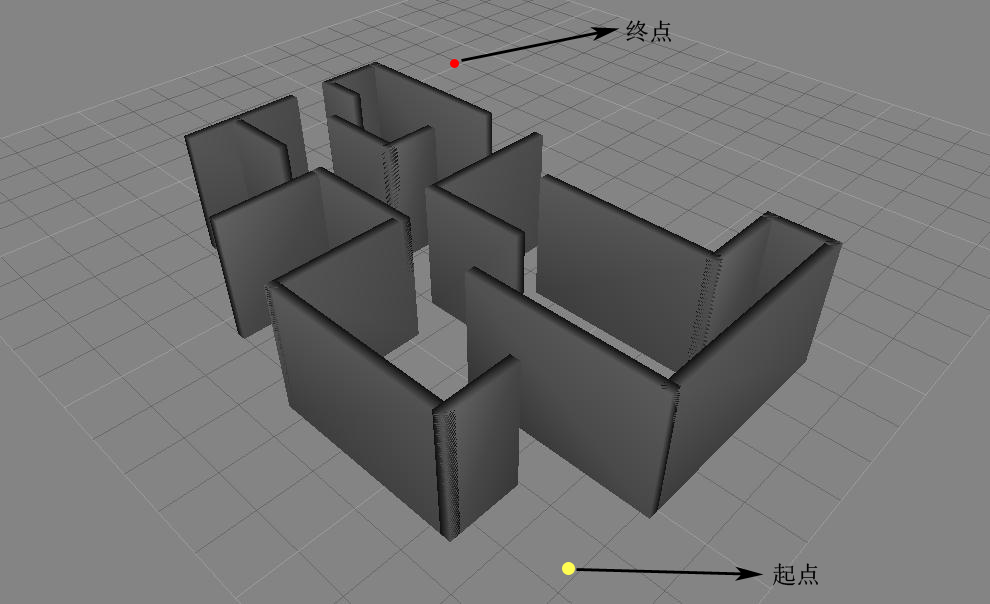
\includegraphics[width=0.8\textwidth]{chap5/Maze.png}
  \bicaption[fig.simWorld]{仿真所建立的障碍物世界}{仿真所建立的障碍物世界}{Fig}{World in simulation}
\end{figure}
\section{机器人的扩展组件撰写}
机器人的扩展组件是指机器人需要实现某一功能而需要拥有的方程文件,GAZEBO支持C++进行组件编写。在本设计中需要通过模型控制文件来实现避障算法。\\
\begin{lstlisting}[language={C}, caption={机器人控制扩展组件}]
#include <boost/bind.hpp>
#include <gazebo.hh>
#include <physics/physics.hh>
#include <sensors/sensors.hh>
#include <common/common.hh>
#include <stdio.h>

namespace gazebo
{   
  class MobileBasePlugin : public ModelPlugin
  {
    public: void Load(physics::ModelPtr _parent, sdf::ElementPtr _sdf) 
    {

      // Store the pointer to the model
      this->model = _parent;

      // Load parameters for this plugin
      if (this->LoadParams(_sdf))
      {
        // testing to see if race condition exists
        gzerr << this->leftWheelJoint->GetAngle(0) << "\n";
        gzerr << this->rightWheelJoint->GetAngle(0) << "\n";
        // Listen to the update event. This event is broadcast every
        // simulation iteration.
        this->updateConnection = event::Events::ConnectWorldUpdateStart(
            boost::bind(&MobileBasePlugin::OnUpdate, this));
      }
    }

    public: bool LoadParams(sdf::ElementPtr _sdf) 
    {

      // Find controller gain
      if (!_sdf->HasElement("gain"))
      {
        gzerr << "param [gain] not found\n";
        return false;
      }
      else
      {
        // Get sensor name
        this->gain =
          _sdf->GetElement("gain")->GetValueDouble();
      }

      // Find sensor name from plugin param
      if (!_sdf->HasElement("ray_sensor"))
      {
        gzerr << "param [ray_sensor] not found\n";
        return false;
      }
      else
      {
        // Get sensor name
        std::string sensorName =
          _sdf->GetElement("ray_sensor")->GetValueString();

        // Get pointer to sensor using the SensorMangaer
        sensors::SensorPtr sensor =
          sensors::SensorManager::Instance()->GetSensor(sensorName);

        if (!sensor)
        {
          gzerr << "sensor by name ["
                << sensorName
                << "] not found in model\n";
          return false;
        }

        this->laser = boost::shared_dynamic_cast<sensors::RaySensor>
          (sensor);
        if (!this->laser)
        {
          gzerr << "laser by name ["
                << sensorName
                << "] not found in model\n";
          return false;
        }
      }

      // Load joints from plugin param
      if (!this->FindJointByParam(_sdf, this->leftWheelJoint,
                             "left_wheel_hinge") ||
          !this->FindJointByParam(_sdf, this->rightWheelJoint,
                             "right_wheel_hinge"))
        return false;

      // success
      return true;
    }

    public: bool FindJointByParam(sdf::ElementPtr _sdf,
                                  physics::JointPtr &_joint,
                                  std::string _param)
    {
      if (!_sdf->HasElement(_param))
      {
        gzerr << "param [" << _param << "] not found\n";
        return false;
      }
      else
      {
        _joint = this->model->GetJoint(
          _sdf->GetElement(_param)->GetValueString());

        if (!_joint)
        {
          gzerr << "joint by name ["
                << _sdf->GetElement(_param)->GetValueString()
                << "] not found in model\n";
          return false;
        }
      }
      return true;
    }

    // Called by the world update start event
    public: void OnUpdate()
    {
      unsigned int n = this->laser->GetRangeCount();
      double min_dist = 1e6;
      for (unsigned int i = 0; i < n; ++i)
      {
        if (this->laser->GetRange(i) < min_dist)
          min_dist = this->laser->GetRange(i);
      }

      double target_dist = 2.0;

      if (min_dist < this->laser->GetRangeMax())
      {
        double torque = this->gain*( min_dist - target_dist );
        this->leftWheelJoint->SetForce(0, torque);
        this->rightWheelJoint->SetForce(0, torque);
      }
    }

    // Pointer to the model
    private: physics::ModelPtr model;

    // Pointer to the update event connection
    private: event::ConnectionPtr updateConnection;

    private: physics::JointPtr leftWheelJoint;
    private: physics::JointPtr rightWheelJoint;
    private: sensors::RaySensorPtr laser;
    private: double gain;
  };

  // Register this plugin with the simulator
  GZ_REGISTER_MODEL_PLUGIN(MobileBasePlugin)
}
\end{lstlisting}
%\section{传感器的扩展组件}
\section{仿真过程与算法验证}
在不断对代码修改后,最终仿真得以实现。仿真截图如图所示。其中蓝色部分为传感器前侧所能感知到的区域,图中车体正在向障碍物间空隙前进。因为在仿真中所计算的数据量非常大,所以仿真速度相对较慢,走出迷宫大概花了25小时46分钟。不过最后小车基本顺利到达指定位置,经测试说明在上章中提出的虚拟势场算法基本可行。
\begin{figure}[!htp]
  \centering
  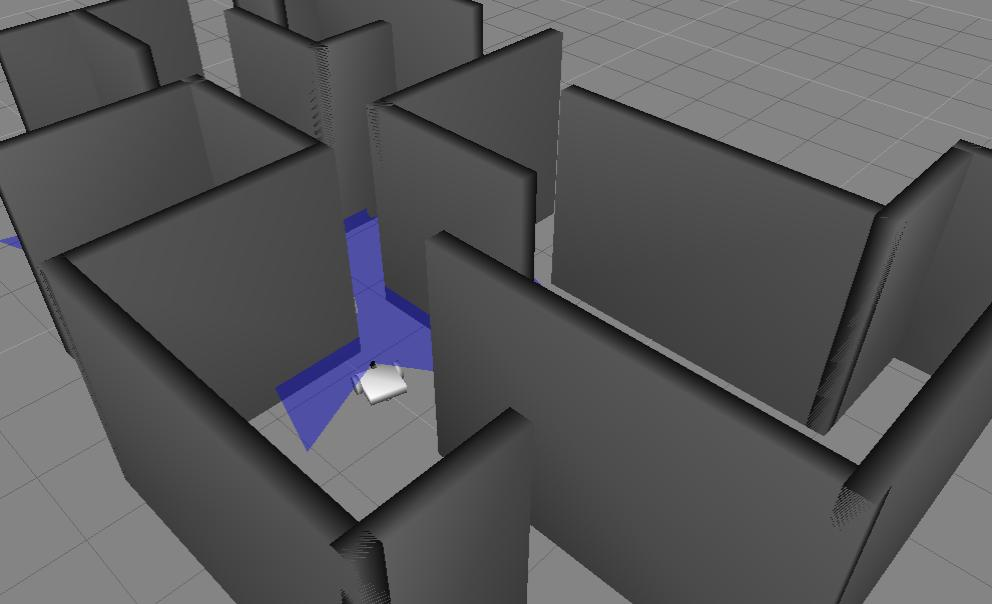
\includegraphics[width=0.8\textwidth]{chap5/OnMoving.jpg}
  \bicaption[fig.simOnMoving]{仿真进行示意图}{仿真进行示意图}{Fig}{The simulation is on going}
\end{figure}

仿真中存在着的问题也比较多,比如算法对于环境还是有一定的依赖性,并不能完全脱离莫一种特定的对环境的要求。所以算法还可以据此进行一些改进。但因为在本设计中使用的环境也即为复杂,而实际中的环境并没有这么复杂,所以说,算法在一般的环境中还是可以正常工作的。所以仿真基本是成功的。而对于这个机器人控制系统的设计也由此基本完成。
\section{本章小结}
本章中详细的介绍了仿真环境的搭建,其中包括模型的创建及生成,传感器的定义与模型体的连接,传感器的信息收集程序,模型的控制程序等。在本节中所验证的算法为上一章所介绍的改良虚拟势场方法。虚拟势场方法在二维环境中,已被多次验证,但在三维环境下被模拟比较少见,而本设计则展示了这一方法的有效性。